\chapter{Propuesta}\label{chapter:proposal}

A partir del estudio hecho en el capítulo anterior podemos asumir que sería beneficioso para las soluciones actuales de código abierto disponer de una API HTTP que permita su configuración de forma programática. Facilitaría la integración con diferentes tipos de interfaces de usuario, ya sea web, de escritorio o una plataforma de terceros. Esta es una característica decisiva para la adopción de más usuarios, por ello los diferentes SaaS apuestan por ella y la ofrecen dentro de sus planes de pago.

Dicha solución sería de especial utilidad en la Universidad de La Habana, institución que por diferentes motivos no hace uso de los SaaS para su solución DNS. En el centro es empleado BIND 9 como servidor de nombres y mantenido por profesionales de la computación en el Nodo UH. Modificaciones básicas, como es añadir un nuevo dominio, serían mucho mas simple a través de una interfaz de usuario. Por lo que una API HTTP compatible con los servidores DNS de código abierto es un paso de avance en el desarrollo de tal objetivo.

De forma subyacente los diferentes servidores de nombres están sujetos a la implementación de DNS propuesta en los RFC. Por tanto, cada uno de los servidores de nombres debe tener el mismo punto de vista respecto al sistema, poseer un sistema de almacenamiento para persistir los diferentes conjuntos de RR en cada zona e implementar las características de DNS actual, tanto las requeridas como las opcionales. Estos puntos en común que deben compartir las diferentes implementaciones de servidores DNS sientan las bases para asumir los aspectos en los que sustentar la propuesta teórica de una API HTTP sobre ellos.

Como propuesta de solución a la implementación de una API para los diferentes softwares de servidores DNS autoritarios de código abierto, se propone un arquitectura en la que la API tiene acceso al sistema de almacenamiento de la configuración DNS para su modificación. Además existe un medio de comunicación entendible por la API y el servidor DNS para desarrollar cualquier intercambio de información necesario.

\begin{figure}[!ht]
    \centering
    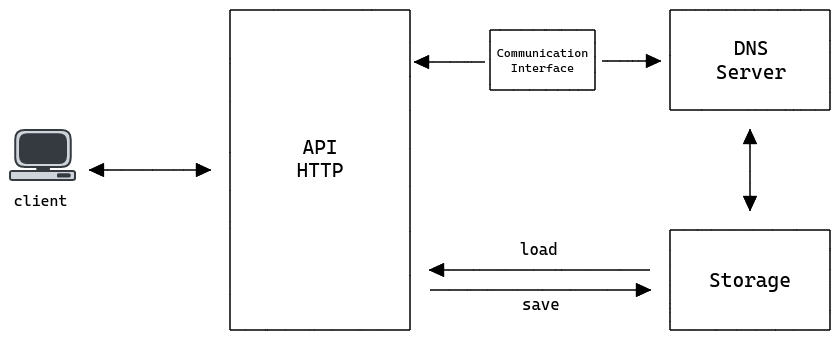
\includegraphics[width=\linewidth]{draws/proposal.png}
    \caption{Arquitectura de la propuesta. La API HTTP sirve como interfaz al sistema de almacenamiento del servidor DNS. Las funciones \textbf{load} y \textbf{save} interactúan de forma directa con el sistema de almacenamiento para leer y escribir la información DNS, respectivamente. La interfaz de comunicación tiene como objetivo poder actualizar o consultar el estado del servidor de forma remota.}
\end{figure}

La hipótesis teórica se basa en dos funciones: \verb+load+ para la lectura de los archivos de configuración desde un sistema de almacenamiento y \verb+save+ para la persistencia de los cambios realizados a dicho sistema. Estas funciones expuestas en una API HTTP, o similar, permiten realizar las funciones fundamentales de configuración sobre el servidor DNS.

En la sección 3.1 se describe el mecanismo de carga de la configuración a través de la función \verb|load|. La sección 3.2 desarrolla el funcionamiento de \verb|save|, cómo esta asegura la correctitud de los cambios realizados en la configuración DNS y notifica al servidor DNS sobre estos.

\section{Lectura de la Configuración DNS}

Asumiendo que existe un servidor DNS autoritario $A$, con un sistema de persistencia en disco $S_A$. Sea $M_A$, la configuración del sistema DNS cargada por la API de $A$ y $r(S_A)$ una función capaz de leer y estructurar la información desde el sistema de almacenamiento $S_A$; se tiene la función \verb+load+ como se muestra a continuación.

\begin{algorithmic}
\Procedure{load}{$A$}
    \State $M_A \leftarrow r(S_A)$
\EndProcedure
\end{algorithmic}

\begin{figure}[!ht]
    \centering
    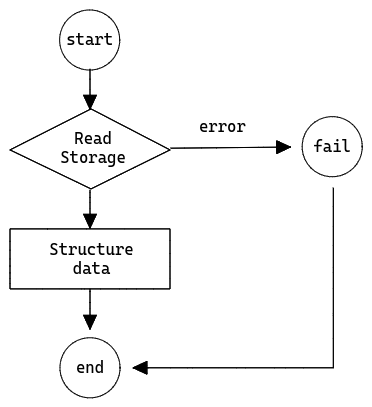
\includegraphics[width=0.5\linewidth]{draws/load.png}
    \caption{Diagrama de flujo para la función \textbf{load}.}
\end{figure}

Este procedimiento tiene como objetivo cargar cada una de las zonas con su conjunto de registros a la API. El mecanismo de lectura debe funcionar de acuerdo a como esta estructurada la información en el servidor DNS: archivos de texto plano, binarios o una base de datos externa. La estructura de datos resultante es manejada por la API y debe reflejar en todo momento el estado actual del servidor DNS.

\section{Escritura de la Configuración DNS}

Para definir \verb+save+, es necesario considerar que existe un mecanismo de comunicación $C_A$ entre el servicio de la API y $A$. Sean $h(C_A)$ una función que indica a $A$ que su configuración en $S_A$ ha sido modificada, $f(M_A, u)$ la función que almacena de forma estructurada en el almacenamiento de la API las modificaciones $u$ enviados a esta y $g(S_A, u)$ la función que persiste el conjunto de modificaciones $u$ de forma estructurada en el sistema de almacenamiento de $A$. Entonces, se define \verb+save+ de la siguiente manera.

\begin{algorithmic}\label{proc:save}
\Procedure{save}{$A$, $u$}
    \State $M_A' \leftarrow f(M_A, u)$
    \State $g(S_A, u)$
    \State $h(C_A)$
    \State $M_A \leftarrow M_A'$
\EndProcedure
\end{algorithmic}

\begin{figure}[!ht]
    \centering
    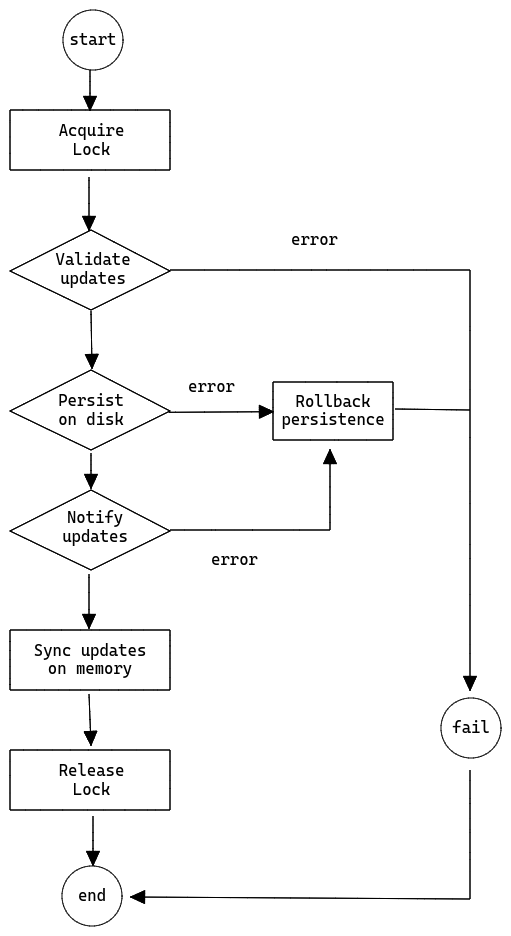
\includegraphics[width=0.6\linewidth]{draws/save.png}
    \caption{Diagrama de flujo para la función \textbf{save}.}
\end{figure}

Cuando se evalúa $f$ son realizadas las validaciones para garantizar que los cambios introducidos por $u$ son compatibles con el estado actual del servidor de nombres $A$. En caso positivo, la actualización introducida por $u$ es persistida. Posteriormente, se notifica al servidor DNS que puede recargar su configuración. Si los estados posteriores (invocación a $g$ y $h$) a la validación de $u$ ocurren sin errores, se actualiza la información en $M_A$ para sincronizarla con los cambios realizados al servidor autoritario $A$.

En caso de errores ambos sistemas deben quedar en el estado anterior a la ejecución de los cambios y la API debe retornar una respuesta indicando el error al completar el pedido. Para ello debe ser implementado un mecanismo que ejecute un \textit{rollback} de forma apropiada.

La interfaz de comunicación es explícitamente necesaria para notificar al servidor DNS de cambios, por lo que cualquier tipo de protocolo factible para este fin es aceptable. En caso que el servidor de nombres sea capaz de detectar cambios en su configuración de forma autónoma en tiempo de ejecución, la invocación a $h$ puede ser omitida en la implementación.

De esta forma, quedan definidas las bases que forman parte de la arquitectura a implementar: una API HTTP que gestiona directamente los archivos de configuración del servidor de nombres a través de dos funciones, \verb|load| y \verb|save|; y un mecanismo de comunicación entre el servicio de la API HTTP y el servidor DNS para notificar de actualizaciones si es necesario. Adicionalmente, la necesidad de un mecanismo para manejar errores y recuperarse de ellos.
